\documentclass[12pt]{scrartcl}
\usepackage[sexy]{james}
\usepackage[noend]{algpseudocode}
\setlength {\marginparwidth}{2cm}
\setcounter{MaxMatrixCols}{20}
\usepackage{answers}
\usepackage{array}
\usepackage{tikz}
\newenvironment{allintypewriter}{\ttfamily}{\par}
\usepackage{listings}
\usepackage{xcolor}
\usetikzlibrary{arrows.meta}
\usepackage{color}
\usepackage{mathtools}
\newcommand{\U}{\mathcal{U}}
\newcommand{\E}{\mathbb{E}}
\usetikzlibrary{arrows}
\Newassociation{hint}{hintitem}{all-hints}
\renewcommand{\solutionextension}{out}
\renewenvironment{hintitem}[1]{\item[\bfseries #1.]}{}
\renewcommand{\O}{\mathcal{O}}
\declaretheorem[style=thmbluebox,name={Chinese Remainder Theorem}]{CRT}
\renewcommand{\theCRT}{\Alph{CRT}}
\setlength\parindent{0pt}
\usepackage{sansmath}
\usepackage{pgfplots}

\usetikzlibrary{automata}
\usetikzlibrary{positioning}  %                 ...positioning nodes
\usetikzlibrary{arrows}       %                 ...customizing arrows
\newcommand{\eqdef}{=\vcentcolon}
\newcommand{\tr}{{\rm tr\ }}
\newcommand{\im}{{\rm Im\ }}
\newcommand{\spann}{{\rm span\ }}
\newcommand{\Col}{{\rm Col\ }}
\newcommand{\Row}{{\rm Row\ }}
\newcommand{\dint}{\displaystyle\int}
\newcommand{\dt}{\ {\rm d }t}
\newcommand{\PP}{\mathbb{P}}
\newcommand{\horizontal}{\par\noindent\rule{\textwidth}{0.4pt}}
\usepackage[top=3cm,left=3cm,right=3cm,bottom=3cm]{geometry}
\newcommand{\mref}[3][red]{\hypersetup{linkcolor=#1}\cref{#2}{#3}\hypersetup{linkcolor=blue}}%<<<changed

\tikzset{node distance=4.5cm, % Minimum distance between two nodes. Change if necessary.
         every state/.style={ % Sets the properties for each state
           semithick,
           fill=cyan!40},
         initial text={},     % No label on start arrow
         double distance=4pt, % Adjust appearance of accept states
         every edge/.style={  % Sets the properties for each transition
         draw,
           ->,>=stealth',     % Makes edges directed with bold arrowheads
           auto,
           semithick}}


% Start of document.
\newcommand{\sep}{\hspace*{.5em}}

\pgfplotsset{compat=1.18}
\begin{document}
\title{MATH403: Homework 5}
\author{James Zhang\thanks{Email: \mailto{jzhang72@terpmail.umd.edu}}}
\date{\today}

\definecolor{dkgreen}{rgb}{0,0.6,0}
\definecolor{gray}{rgb}{0.5,0.5,0.5}
\definecolor{mauve}{rgb}{0.58,0,0.82}

\lstset{frame=tb,
  language=Java,
  aboveskip=3mm,
  belowskip=3mm,
  showstringspaces=false,
  columns=flexible,
  basicstyle={\small\ttfamily},
  numbers=left,
  numberstyle=\tiny\color{gray},
  keywordstyle=\color{blue},
  commentstyle=\color{dkgreen},
  stringstyle=\color{mauve},
  breaklines=true,
  breakatwhitespace=true,
  tabsize=3
}

\maketitle

\begin{center}
  
\includegraphics[width=13cm]{6.png}
\end{center}
\begin{proof}
  COsndier $G = S_3$, the symmetric group of 3 elements. $G$ contains the followng elements 
  \[G = \{e, (12), (13), (23), (123), (132)\}\]
  Now suppose we define the following subgroups 
  \begin{align*}
    H = \{e, (12)\} && K = \{e, (13)\}
  \end{align*}
  Observe that 
  \[HK = \{e, (12), (13), (12)(13)\} = \{e, (12, (13), (132))\}\]
  However, $(13)(132) = (23)$ which isn't in $HK$, and so $HK$ is not closed and so it 
  is not a subgroup, even though $H$ and $K$ are. 
\end{proof}
\newpage

\begin{center}
  
\includegraphics[width=13cm]{8.png}
\end{center}
\begin{proof}
  \hfill

  $\Longrightarrow$ Let us show that $H \subseteq K$. Let $x \in H$. By \textbf{Property 1 of Lemma 7.1}, 
  $ax \in aH$. Since $aH = bK \implies ax \in bK$. Furthermore, observe that 
  \[a \in aH \implies ae \in aH \implies a \in bK \implies a^{-1} \in bK\]
  and $b = be \in bK$. By \textbf{Property 9 of Lemma 7.1}, $bK$ is a subgroup of $G$ because 
  $b \in G$. Now see that 
  \[x = a^{-1}ax \in bK \implies bx \in bK \implies x \in K\]
  as desired, and the first step above is by closure. Thus, $H \subseteq K$. 
  
  \hfill

  $\Longleftarrow$ The proof in the other direction is very similar to show that $K \subseteq H$. Simply replace 
  all $a$ with $b$ and vice versa and $H$ with $K$ and vice versa. 

  \hfill
  
  Thus, $H = K$, as desired. 
\end{proof}
\newpage

\begin{center}
  
\includegraphics[width=13cm]{10.png}
\end{center}
\begin{proof}
  Let $a, b \in H$ where $a, b \neq e$, $|a| \neq |e|$, $H \subseteq G$, and $|G| = 155$. We want to show that 
  $H$ must be $G$. Note that the order of $G$ is finite because $|G| = 155$ and $H \subseteq G$. Therefore, 
  by \textbf{Lagrange's Theorem}, $|H| \slash |G|$. The only posiitive divisors of $155$ are $1 5, 31, 155$. Therefore, 
  \[|H| \in \{1, 5, 31, 155\}\]
  Note that $e, a, b \in H$ is given, so $|H| \neq 1$. Now suppose $|H| = 5$. Then by \textbf{Corollary 2} which states that in a finite group, 
  the order of each element of the group divides the order of the group, this implies that 
  $|a| \slash |H|$ and $|b| \slash |H|$, and therefore, $|a|, |b| \in \{1, 5\}$. However, 
  $a \neq e$ and $b \neq e$ which implies that $|a| = 5$ and $|b| = 5$, which contradicts the given statement that 
  $a$ and $b$ are of different orders. A similar argument can be applied to show that $|H| \neq 31$ because 
  $31$ is also prime. Therefore, $|H| = 155$, and since $H \subseteq G \implies H = G$ must be true, and so the only 
  subgrouo of $G$ that contains $a$ and $b$ is $G$ itself, as desired.
\end{proof}
\newpage

\begin{center}
  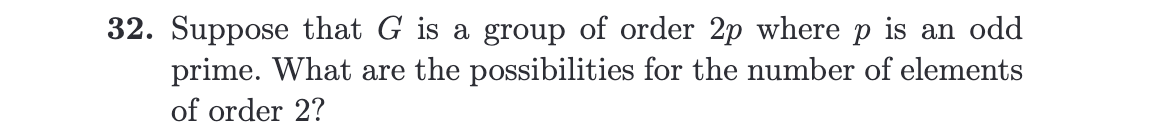
\includegraphics[width=13cm]{32.png}
\end{center}
\begin{proof}
  By \textbf{Theorem 7.3}, $G$ is isomorphic to $\ZZ_{2p}$ or $D_p$. Let's proceed by taking cases. 
  Note that isomorphisms preserve order. 
  \begin{enumerate}[(i)]
    \item Suppose $G \approx \ZZ_{2p}$. Note that the only element of order $2$ in $\ZZ_{2p}$ is $p$, and so the number of elements of order $2$ are 
    $1$. 
    \item Suppose $G \approx D_p$. Note that $D_p$ consists of $p$ reflections and $p$ rotations. The only rotation of order $2$
    is 180 degrees, and all reflections have order $2$. Thus, the number of elements of order $2$ are $p + 1$. 
  \end{enumerate}
\end{proof}
\newpage

\begin{center}
  
\includegraphics[width=13cm]{42.png}
\end{center}
\begin{proof}
  Let $G$ be a group of order $63$, which is finite. We want to show that there exists some element $a \in G$ 
  such that $|a| = 3$, so on the contrary, assume that there does not exist an element of order $3$. 
  By \textbf{Corollary 2}, $|a| \slash 63$. Therefore, 
  \[|a| \in \{1, 3, 7, 9, 21, 63\}\]
  Note that $|a| = 1 \implies a = e$, which doesn't have order $3$. We assume that 
  $\not\exists a \in G$ s.t. $|a| = 3$. Further observe that $|a| \neq 9$ because 
  because then the element $|a^3| = 3$, which contradicts our given assertion. The same argument can be applied to $21$ and $63$ because then 
  $|a^7| = 3$ and $|a^{21}| = 3$. Therefore, the order of $a$ must be $7$ for all elements in $G \backslash \{e\}$. 
  Note that $|G \backslash \{e\}| = 62$. 
  By \textbf{Corollary 4.1}, the number of elements of order $7$ in $G \backslash \{e\} \implies |G \backslash \{e\}| = 62$
  must be a multiple of $\phi(7) = 6$. However, $62$ is not a multiple of $6$, and so we have arrived at a contradiction. Therefore, 
  there exists an element $a$ of order $3$ in $G$. 
\end{proof}
\newpage

\begin{center}
  
\includegraphics[width=13cm]{62.png}
\end{center}
\begin{proof}
  Note that $A_5$ is the alternating group of even permutations on 5 elements. For each permutation to be even, 
  there must be an even number of 2-cycles. Therefore, the elements of $A_5$ can be
  \begin{itemize}
    \item The identity $\implies$ 1 of these
    \item 3-cycles $\implies \binom{5}{3} * 2 = 20$ of these
    \item 5-cycles $\implies \binom{5!}{5} = 24$ of these
    \item Disjoint 2-cycles $\implies \frac{5!}{2^2 * 2! * 1} = 15$ of these
  \end{itemize}
  and we confirm for our sanity that this does sum to $60$, the total number of elements in $A_5$. Now, on the contrary, 
  suppose that there is a subgroup $H$ of order $20$ in $A_5$. Consider $a \notin H, |a| = 5$. Our aim is to show that 
  every element of order $5$ is in $H$. As there are $24$ 5-cycles, this will prove that our assumption is wrong in this case. 
  We can decompose $A_5$ into the disjoint union of cosets 
  \[A_5 = H \cup aH \cup a^2H\]
  Now consider the element $a^3$, which must be in $A_5$, and therefore must be in either $H, aH$, or $a^2H$. 
  \begin{itemize}
    \item Suppose $a^3 \in H \implies (a^3)^2 \in H \implies a^6 = a \in H$, which is a contradiction
    \item Suppose $a^3 \in aH \implies a^2 \in H \implies (a^2)^3 = a^6 = a \in H$, which is a contradiction
    \item Suppose $a^3 \in a^2H \implies a^{-2}a^3 \in a^{-2}a^2 \in H \implies a \in H$, which is a contradiction.
  \end{itemize}
  Thus, $a^3 \not\in A_5$, which itself is a contradiction, and this means $a \in H$ for all 5-cycles $a$. Therefore, 
  considering only 5-cycles, $|H| \geq 24$ (not including the identity) and so $H$ cannot be of order $15$ or $20$, as desired.
\end{proof}
\end{document}

